% ============================================================
% TempoRAG-KG — TikZ Figures
% Copy each figure block to replace the \fbox{} placeholder
% in temporag_kg_report.tex
% ============================================================

% Add these packages at the top of your main .tex file:
% \usepackage{tikz}
% \usepackage{pgfplots}
% \pgfplotsset{compat=1.18}
% \usetikzlibrary{arrows.meta, positioning, shapes.geometric, fit, backgrounds, calc}

% ============================================================
% FIGURE 1 — System Architecture
% Replace the \fbox{...} inside \begin{figure*}[t]
% ============================================================

\begin{tikzpicture}[
  font=\small,
  box/.style={rectangle, rounded corners=3pt, draw=#1!70, fill=#1!15,
              text centered, minimum height=0.7cm, minimum width=2.2cm,
              inner sep=4pt},
  ourbox/.style={rectangle, rounded corners=3pt, draw=blue!70, fill=blue!20,
                 text centered, minimum height=0.7cm, minimum width=2.2cm,
                 inner sep=4pt, font=\small\bfseries},
  arr/.style={-{Stealth[length=5pt]}, thick, gray!70},
  ourarr/.style={-{Stealth[length=5pt]}, thick, blue!60},
  label/.style={font=\footnotesize\itshape, text=gray!80}
]

%% ---- OFFLINE PIPELINE (top row) ----
\node[label] at (0, 0.6) {Offline Pipeline};

\node[box=gray] (docs)    at (0, 0)       {Documents};
\node[box=gray] (chunk)   at (2.6, 0)     {Chunking\\{\tiny 512 tok, 100 overlap}};
\node[ourbox]   (extract) at (5.8, 0)     {LLM Extraction\\{\tiny +valid\_from/valid\_to}};
\node[ourbox]   (neo4j)   at (9.0, 0)     {Neo4j KG\\{\tiny temporal edges}};
\node[box=gray] (faiss)   at (9.0, -1.2)  {FAISS Index\\{\tiny entity embeddings}};

\draw[arr]    (docs)    -- (chunk);
\draw[arr]    (chunk)   -- (extract);
\draw[ourarr] (extract) -- (neo4j);
\draw[arr]    (extract) -- ++(0,-0.6) -| (faiss);

%% ---- ONLINE PIPELINE (bottom rows) ----
\node[label] at (0, -2.6) {Online Pipeline};

\node[box=gray] (query)   at (0, -3.3)    {User Query};
\node[ourbox]   (detect)  at (2.4, -3.3)  {Temporal\\Detection ($y_q$)};
\node[box=gray] (seed)    at (4.8, -3.3)  {Seed Retrieval\\{\tiny FAISS top-5}};
\node[ourbox]   (filter)  at (7.2, -3.3)  {Temporal\\Filter (Eq.1)};
\node[box=gray] (gear)    at (9.6, -3.3)  {GEAR Beam\\Search};
\node[ourbox]   (gog)     at (9.6, -4.7)  {GoG Fill-in\\{\tiny if dead end}};
\node[box=gray] (mst)     at (7.2, -4.7)  {MST Context\\Organization};
\node[box=gray] (llm)     at (4.8, -4.7)  {LLM\\Generation};
\node[box=gray] (ans)     at (2.4, -4.7)  {Answer};

\draw[ourarr] (query)  -- (detect);
\draw[ourarr] (detect) -- (seed);
\draw[ourarr] (seed)   -- (filter);
\draw[ourarr] (filter) -- (gear);
\draw[arr]    (gear)   -- (gog);
\draw[arr]    (gog)    -- (mst);
\draw[arr]    (mst)    -- (llm);
\draw[arr]    (llm)    -- (ans);

%% ---- Legend ----
\node[ourbox, minimum width=1.4cm] (leg1) at (6.0, -6.0) {Our addition};
\node[box=gray, minimum width=1.4cm, right=0.3cm of leg1] (leg2) {KG$^2$RAG};
\node[font=\footnotesize, left=0.1cm of leg1] {Legend:};

\end{tikzpicture}


% ============================================================
% FIGURE 2 — Temporal Failure Taxonomy (2x2 grid)
% Replace the \fbox{...} inside \begin{figure}[t]
% ============================================================

\begin{tikzpicture}[
  font=\small,
  cell/.style={rectangle, rounded corners=4pt, draw=#1!60, fill=#1!10,
               minimum width=4.6cm, minimum height=2.8cm,
               align=center, inner sep=6pt},
  tag/.style={rectangle, rounded corners=2pt, fill=#1!70,
              text=white, font=\footnotesize\bfseries, inner sep=3pt}
]

%% Top-left: Type 1
\node[cell=red]   (t1) at (0, 0)    {
  \textbf{Type 1 — Stale Fact}\\[4pt]
  KG retrieves expired fact\\
  as if currently valid\\[4pt]
  \textit{\footnotesize ``Steve Jobs'' as\\current Apple CEO}
};
\node[tag=red, anchor=north west] at (t1.north west) {Type 1};

%% Top-right: Type 2
\node[cell=orange] (t2) at (5.0, 0) {
  \textbf{Type 2 — Conflicting Facts}\\[4pt]
  Multiple contradictory facts\\
  retrieved simultaneously\\[4pt]
  \textit{\footnotesize Both Jobs and Cook\\returned as CEO}
};
\node[tag=orange, anchor=north west] at (t2.north west) {Type 2};

%% Bottom-left: Type 3
\node[cell=blue]  (t3) at (0, -3.4) {
  \textbf{Type 3 — Missing Context}\\[4pt]
  Correct entity retrieved,\\
  validity window unknown\\[4pt]
  \textit{\footnotesize Cook is CEO,\\but which years?}
};
\node[tag=blue, anchor=north west] at (t3.north west) {Type 3};

%% Bottom-right: Type 4
\node[cell=violet] (t4) at (5.0, -3.4) {
  \textbf{Type 4 — Hop Failure}\\[4pt]
  Stale fact at any hop\\
  breaks the reasoning chain\\[4pt]
  \textit{\footnotesize Hop 1 correct;\\hop 2 retrieves outdated}
};
\node[tag=violet, anchor=north west] at (t4.north west) {Type 4};

%% Axis labels
\node[font=\footnotesize\bfseries, rotate=90] at (-2.8, -1.7) {Single-hop};
\node[font=\footnotesize\bfseries, rotate=90] at (-2.8,  0.0) {Single-hop};

\end{tikzpicture}


% ============================================================
% FIGURE 3 — Expected Ablation Results (bar chart)
% Replace the \fbox{...} inside the Expected Results section
% ============================================================

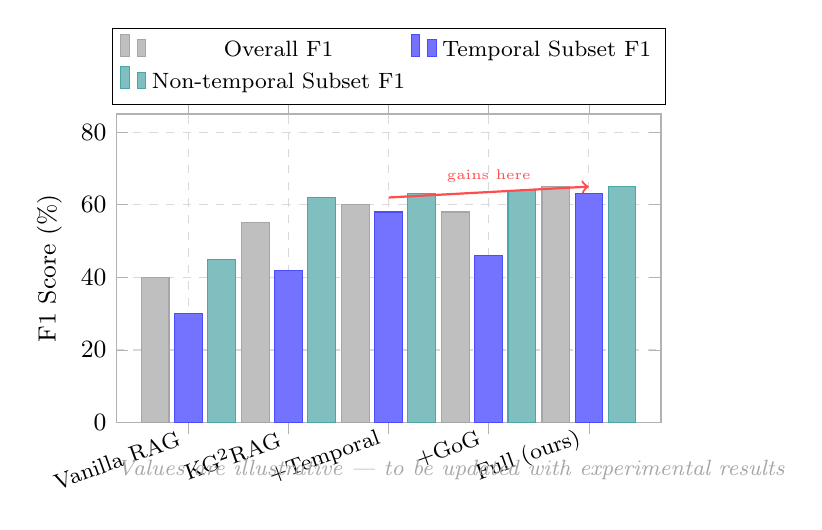
\begin{tikzpicture}
\begin{axis}[
  ybar,
  bar width=0.35cm,
  width=8.5cm,
  height=5.5cm,
  enlarge x limits=0.18,
  legend style={
    at={(0.5,1.03)},
    anchor=south,
    legend columns=2,
    font=\footnotesize
  },
  ylabel={F1 Score (\%)},
  ylabel style={font=\small},
  symbolic x coords={
    {Vanilla RAG},
    {KG$^2$RAG},
    {+Temporal},
    {+GoG},
    {Full (ours)}
  },
  xtick=data,
  x tick label style={font=\footnotesize, rotate=20, anchor=east},
  ymin=0, ymax=85,
  ytick={0,20,40,60,80},
  yticklabel style={font=\small},
  grid=major,
  grid style={dashed, gray!30},
  axis line style={gray!60},
  tick style={gray!60},
  nodes near coords style={font=\tiny, /pgf/number format/fixed},
]

%% Overall F1 (gray bars — placeholder values showing expected trend)
\addplot[fill=gray!50, draw=gray!70]
  coordinates {
    ({Vanilla RAG},     40)
    ({KG$^2$RAG},       55)
    ({+Temporal},       60)
    ({+GoG},            58)
    ({Full (ours)},     65)
  };

%% Temporal Subset F1 (blue bars — bigger improvement expected)
\addplot[fill=blue!55, draw=blue!70]
  coordinates {
    ({Vanilla RAG},     30)
    ({KG$^2$RAG},       42)
    ({+Temporal},       58)
    ({+GoG},            46)
    ({Full (ours)},     63)
  };

%% Non-temporal Subset F1 (green bars — expected to stay flat)
\addplot[fill=teal!50, draw=teal!70]
  coordinates {
    ({Vanilla RAG},     45)
    ({KG$^2$RAG},       62)
    ({+Temporal},       63)
    ({+GoG},            64)
    ({Full (ours)},     65)
  };

\legend{Overall F1, Temporal Subset F1, Non-temporal Subset F1}

%% Annotation: expected gain on temporal
\draw[->, red!70, thick] (axis cs:{+Temporal}, 62) -- (axis cs:{Full (ours)}, 65)
  node[midway, above, font=\tiny, text=red!70] {gains here};

\end{axis}

%% Note below chart
\node[font=\footnotesize\itshape, text=gray!70, align=center]
  at (4.25, -0.6) {Values are illustrative — to be updated with experimental results};

\end{tikzpicture}

